\chapter{Task 49: Temporal winner-loser networks}

\resp{Andrea Santarossa}

\noindent\textcolor{unipd}{\textit{Temporal winner-loser networks in WWE, tennis, and football.}}

This project focuses on the reconstruction of temporal winner--loser networks in WWE/WWF, tennis, and international football, representing competitive interactions as directed weighted graphs aggregated into four-month snapshots. The main WWE/WWF dataset was obtained from Kaggle \cite{wwe_dataset}, while ATP and WTA tennis results were collected from the Jeff Sackmann repositories \cite{atp_dataset,wta_dataset}. International football match data were retrieved from the historical results repository by Mart Jürisoo \cite{football_dataset}. The aim of the project is to compare the temporal evolution of dominance, centrality, and interaction patterns across sports characterized by different competitive structures through the construction of temporal multilayer networks.


\section{Data Preprocessing Pipeline}

The preprocessing pipeline follows a similar structure across the three datasets. First, raw match records are imported and cleaned by removing missing or invalid values, while draws are excluded from the football network construction. For the \texttt{WWE/WWF} dataset, only 
\texttt{WWE}, \texttt{WWF}, \texttt{WWWF}, \texttt{WCW}, \texttt{ECW}, and \texttt{NXT}
promotions are retained. In addition, matches labelled as \texttt{battle royal}, \texttt{royal rumble}, \texttt{gauntlet}, \texttt{casino}, \texttt{bunkhouse}, \texttt{elimination chamber}, \texttt{rumble}, and \texttt{battle royale} are excluded from the winner--loser network, since these match types involve complex all-versus-all elimination dynamics where interpreting the final winner as having directly defeated every participant could artificially inflate the number of winner--loser interactions generated by a single event. Matches are then classified into the interaction layers \texttt{singles}, \texttt{tag\_team}, and \texttt{multi\_person}.

After the cleaning phase, directed winner--loser edges are created by connecting each winner to the corresponding loser(s), such that an edge $A \rightarrow B$ indicates that player (or team) $A$ defeated player (or team) $B$. In wrestling, edge construction depends on the match layer, while in tennis and football each match produces a single directed interaction between competitors. Match dates are then converted into temporal snapshots using fixed four-month windows (\texttt{January--April}, \texttt{May--August}, and \texttt{September--December}), allowing interactions occurring within the same period to be aggregated together. Finally, edge weights are summed within each snapshot in order to construct the final temporal weighted networks.

The resulting preprocessed networks are stored in CSV files with a standardized edge-list representation:

\begin{itemize}
    \item \colorbox{gray!15}{\texttt{wrestling\_network.csv}}: \texttt{source}, \texttt{target}, \texttt{weight}, \texttt{snapshot\_start}, \texttt{snapshot\_end}, \texttt{year}, \texttt{promotion}, \texttt{organization\_group}, \texttt{layer}.

    \item \colorbox{gray!15}{\texttt{tennis\_network.csv}}: \texttt{source}, \texttt{target}, \texttt{weight}, \texttt{snapshot\_start}, \texttt{snapshot\_end}, \texttt{tour}.
    
    \item \colorbox{gray!15}{\texttt{football\_network.csv}}: \texttt{source}, \texttt{target}, \texttt{weight}, \texttt{snapshot\_start}, \texttt{snapshot\_end}, \texttt{tournament}.
\end{itemize}

\begin{table}[h]
\centering
\begin{tabular}{lcccc}
\hline
\textbf{Dataset} & \textbf{Interactions} & \textbf{Snapshots} & \textbf{Unique Nodes} & \textbf{Time Span} \\
\hline
Wrestling & 124961 & 189 & 5932 & 1963--2026 \\
Tennis & 1699267 & 343 & 65004 & 1877--2026 \\
Football & 36057 & 400 & 335 & 1873--2026 \\
\hline
\end{tabular}
\caption{Summary statistics of the temporal network datasets. \textit{Interactions} indicates the total number of edges, \textit{Snapshots} the number of temporal snapshots, \textit{Unique Nodes} the total number of distinct nodes, and \textit{Time Span} the period between the first and last snapshot.}
\label{tab:dataset_summary}
\end{table}


\section{Network analysis}

In Appendix~\ref{app:temp_network} are reported the plots showing the temporal evolution of the network structure. In particular, the evolution of the number of nodes and edges across snapshots is analyzed to characterize long-term structural changes in the three sports systems. 

Starting from wrestling, the number of nodes remains relatively stable over time, indicating a consistent pool of active wrestlers across decades, while the number of edges shows an oscillatory behavior with alternating phases of increase and decrease. In tennis, a different pattern emerges, with a clear and persistent increase in the number of edges starting from the 1960s, reflecting the expansion of the professional circuit and the growing number of tournaments. The number of nodes increases only moderately, suggesting that growth is mainly driven by higher match frequency rather than a larger player base. Finally, football exhibits the strongest structural growth, with both nodes and edges increasing significantly over time, especially from the 1960s onward, reflecting the expansion of international competitions and participating national teams.

In Appendix~\ref{app:den_com_cen} are reported the plots describing additional structural properties, including density, number of communities, and centrality. Density captures the overall level of interconnectedness of the system, while the number of communities, computed via greedy modularity on the undirected version of the network, reflects its internal organization into competitive clusters. Centrality is measured using \texttt{PageRank} on the reversed directed network, ensuring that importance flows from defeated opponents toward dominant competitors.

The dominance measure is defined as the number of snapshots in which each player (or team) attains the highest \texttt{PageRank} score, providing a notion of sustained superiority over time. In addition, the temporal evolution of rankings is analyzed by tracking the rank trajectories of the top five players over time. The corresponding results are reported in Figure~\ref{fig:wrestling_rank_evolution}, Figure~\ref{fig:tennis_rank_evolution}, and Figure~\ref{fig:football_rank_evolution} for wrestling, tennis, and football respectively. In wrestling, a clear long-term dominance emerges for \textit{Bruno Sammartino} during the 1960s–1980s, while in more recent years dominance appears more fragmented among \textit{Randy Orton}, \textit{John Cena}, and \textit{The Undertaker}. In tennis, the post-2000 era is characterized by a strong rivalry between \textit{Novak Djokovic} and \textit{Roger Federer}, which largely defines the competitive hierarchy of the period. In football, early records (pre-1900) show a clear dominance of \textit{England}, while in the modern era (2000s) a strong superiority of \textit{Brazil} emerges in terms of sustained performance.

Finally, Appendix~\ref{app:dom-rank} reports a more detailed breakdown of dominance and rank evolution across different layers of the wrestling dataset, different circuits in tennis, and different tournaments in football.


% WRESTLING
\begin{figure}[!htbp]
    \centering

    \makebox[\textwidth][c]{%
        \begin{minipage}{1.18\textwidth}
            \centering
            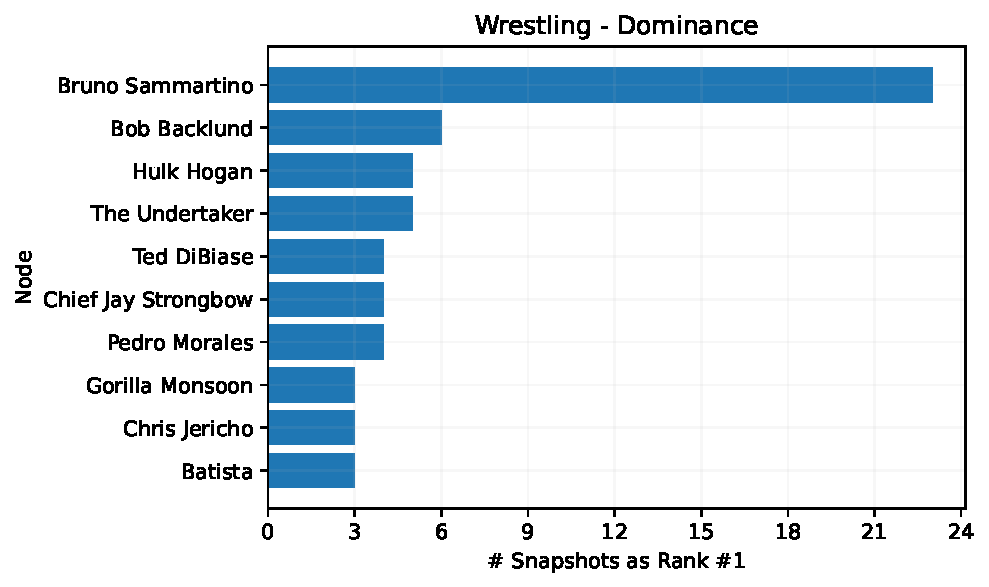
\includegraphics[width=0.39\textwidth]{plots/Wrestling_dominance.pdf}
            \hspace{0.0\textwidth}
            \raisebox{0.cm}{
                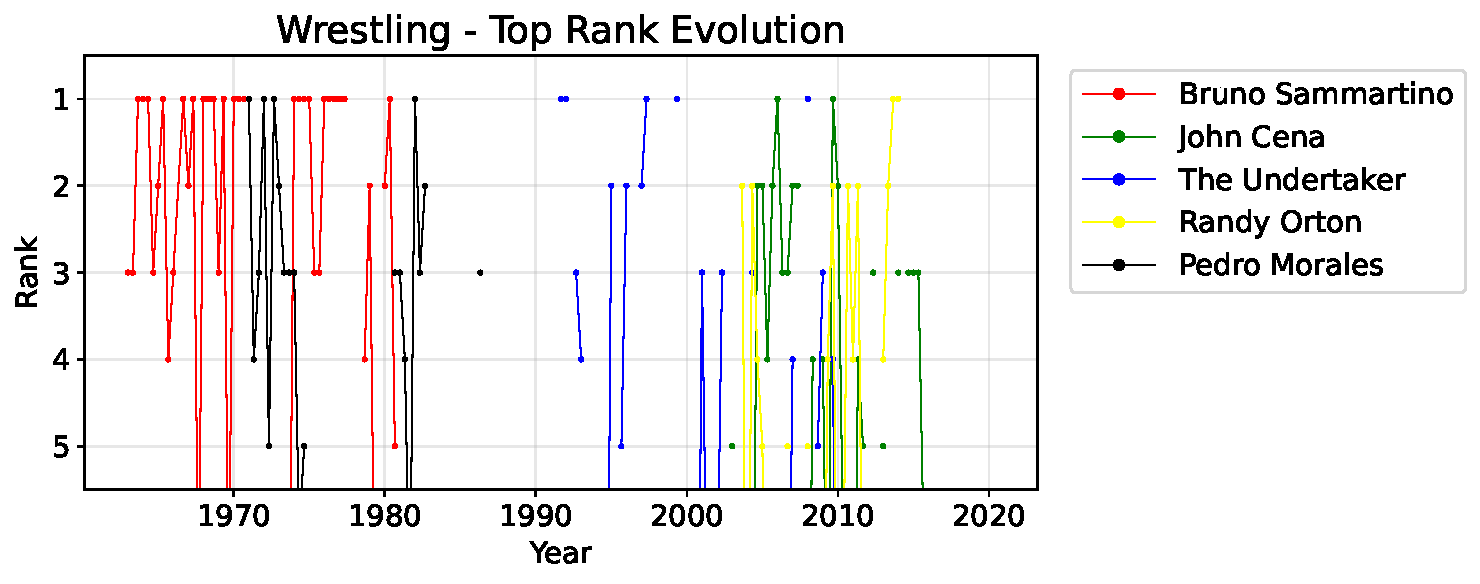
\includegraphics[width=0.58\textwidth]{plots/Wrestling_rank_evolution.pdf}
            }
        \end{minipage}
    }

    \captionsetup{
        width=1.15\textwidth,
        font={footnotesize,stretch=0.9},
        labelfont=bf,
        skip=2pt
    }

    \caption{Wrestling. Distribution of dominance scores and temporal evolution of ranks over the complete dataset.}
    \label{fig:wrestling_rank_evolution}
\end{figure}

% TENNIS
\begin{figure}[!htbp]
    \centering

    \makebox[\textwidth][c]{%
        \begin{minipage}{1.18\textwidth}
            \centering
            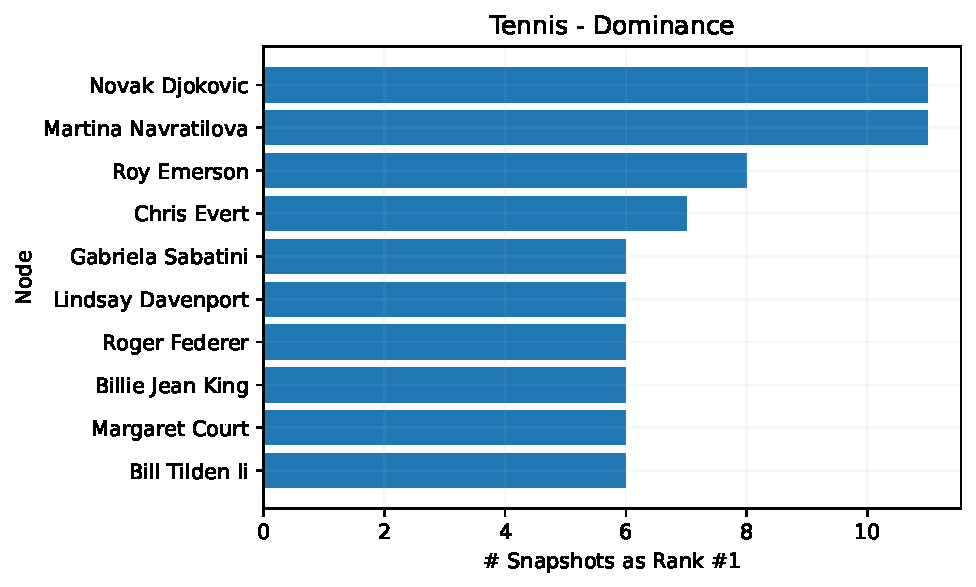
\includegraphics[width=0.39\textwidth]{plots/Tennis_dominance.pdf}
            \hspace{0.0\textwidth}
            \raisebox{0.cm}{
                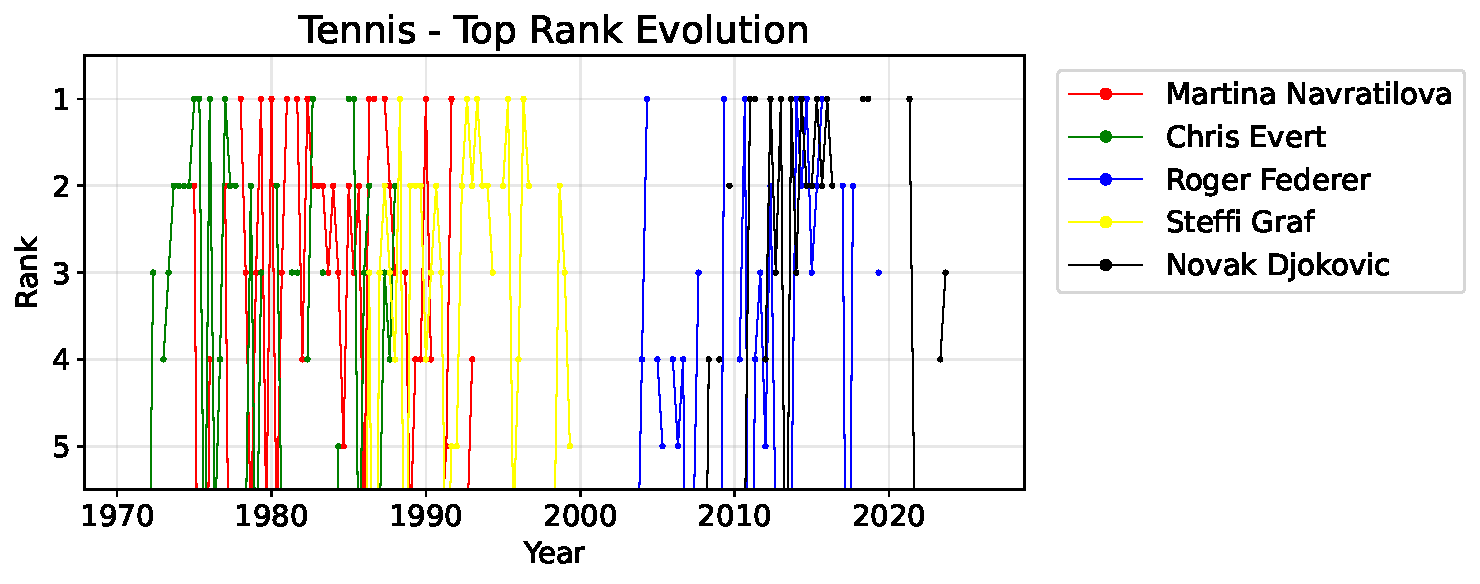
\includegraphics[width=0.58\textwidth]{plots/Tennis_rank_evolution.pdf}
            }
        \end{minipage}
    }

    \captionsetup{
        width=1.15\textwidth,
        font={footnotesize,stretch=0.9},
        labelfont=bf,
        skip=2pt
    }

    \caption{Tennis. Distribution of dominance scores and temporal evolution of ranks over the complete dataset.}
    \label{fig:tennis_rank_evolution}
\end{figure}

% FOOTBALL
\begin{figure}[!htbp]
    \centering

    \makebox[\textwidth][c]{%
        \begin{minipage}{1.18\textwidth}
            \centering
            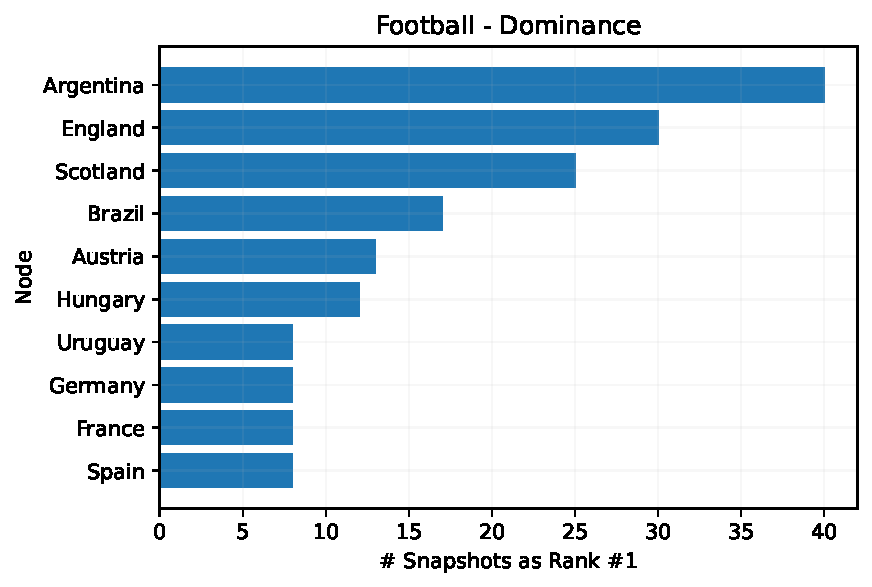
\includegraphics[width=0.39\textwidth]{plots/Football_dominance.pdf}
            \hspace{0.0\textwidth}
            \raisebox{0.3cm}{
                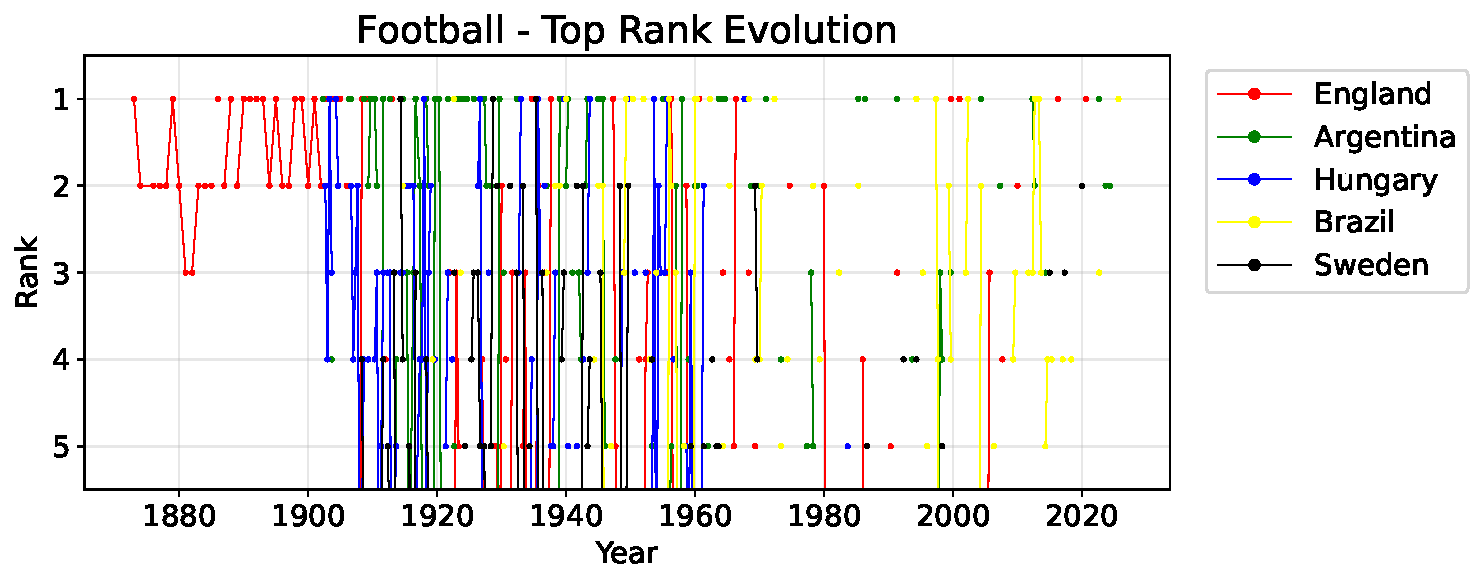
\includegraphics[width=0.58\textwidth]{plots/Football_rank_evolution.pdf}
            }
        \end{minipage}
    }

    \captionsetup{
        width=1.15\textwidth,
        font={footnotesize,stretch=0.9},
        labelfont=bf,
        skip=2pt
    }

    \caption{Football. Distribution of dominance scores and temporal evolution of ranks over the complete dataset.}
    \label{fig:football_rank_evolution}
    
\end{figure}

\newpage